\section{Results}

In this section we investigate the support for the hypotheses outlined in \cref{sec:intro}. 
We test hypothesis \ref{asmpt:rf-first} in \cref{ssec:results-stacking}, then informed on those results, we examine hypothesis \ref{asmpt:represent} in \cref{ssec:res-latents}.
We then investigate hypothesis \ref{asmpt:lang-mod} in \cref{ssec:results-lm}, provide a discussion of hypothesis \ref{asmpt:end2end}, and re-investigate hypothesis \ref{asmpt:represent} in \cref{ssec:results-asr}.

\subsection{Expanding the receptive field of WaveNet by stacking}\label{ssec:results-stacking}
\begin{table}[t]
    \centering
    \begin{tabular}{l l r | r ||r}
    
    S & N & C & RF (ms) & BPD \\ \hline
    2 & 5 & 64 & 10234 (640)  & \textbf{11.835}        \\  % https://wandb.ai/vseq/wavenet/runs/tzusj8ta
    4 & 5 & 64 &  20468 (1280) & 12.331                \\  % https://wandb.ai/vseq/wavenet/runs/cgjagosy
    8 & 5 & 64 &  40936 (2560) & 12.621                \\  % https://wandb.ai/vseq/wavenet/runs/3b8px7kn
    16 & 5 & 64 & 81872 (5120) & 13.060                \\  % https://wandb.ai/vseq/wavenet/runs/7zue6qqs
    \hline
    2 & 5 & 92 &  10234 (640)  &  11.878    \\ 
    4 & 5 & 92 &  20468 (1280) &  12.249    \\ 
    8 & 5 & 92 &  40936 (2560) &  12.503    \\ 
    16 & 5 & 92 & 81872 (5120) & 12.861     \\ 
    % 2 & 4 & t 92 & 8188 & 11.718      \\ 
    \hline
    2 & 1 & 128 & 2050 (128) & 12.156     \\ 
    4 & 1 & 128 & 4100 (256) & 12.312     \\ 
    8 & 1 & 128 & 8200 (512) & 12.740     \\ 
    16 & 1 & 128 & 16400 (1025) & 13.042    \\ 
    \hspace{0.5cm}
    \end{tabular}
    \caption{BPD for WaveNet on TIMIT Test set for 50 epochs. 
    All Residual Stacks have 10 layers with exponentially increasing dilation, i.e. for layer $i$ the dilation will be $d_i = 2^{i}, i \in {1, 10}$
    }
    \label{tab:stack-bpds}
\end{table}

To test hypothesis \ref{asmpt:rf-first}, that a larger receptive field will increase the predictive power of a WaveNet, we trained WaveNets with different stacking setups.
The results are shown in \cref{tab:stack-bpds}.

From these, we report the following:
\paragraph{Increasing the stacking does not improve likelihoods significantly.}
This result opposes hypothesis \ref{asmpt:rf-first}, hinting that the information within the Receptive Field of the original WaveNet is sufficient for generating high-fidelity audio.

\paragraph{Increasing the number of residual channels} from 64 to 92 channels \textbf{increases} evaluation likelihoods for higher stacks, but \textbf{decreases} evaluation likelihoods for 2-stacks. We infer that the limiting factor in WaveNets with larger stack sizes is the number of information channels, not the size of the receptive field. 

\paragraph{Generated audio} from the "stacked" WaveNet (can be found \href{https://magnus.sletfjerding.no/publication/msc-thesis/}{here}) \textit{still} sounds like babbling; we observe no significant improvement in the coherence of syllables or words. 

This result hints that the WaveNet does not capture sufficient semantic information from its inputs, even with a receptive field of multiple seconds. 
Whether this presents a fundamental architectural limit to convolutional autoregressive  models remains unknown to us at this time.
% TODO: mention deeper architectures?

\subsection{Latent space of Stacked WaveNet output space}\label{ssec:res-latents}
\begin{figure}[htb]
    \centering
    % \subfloat{
        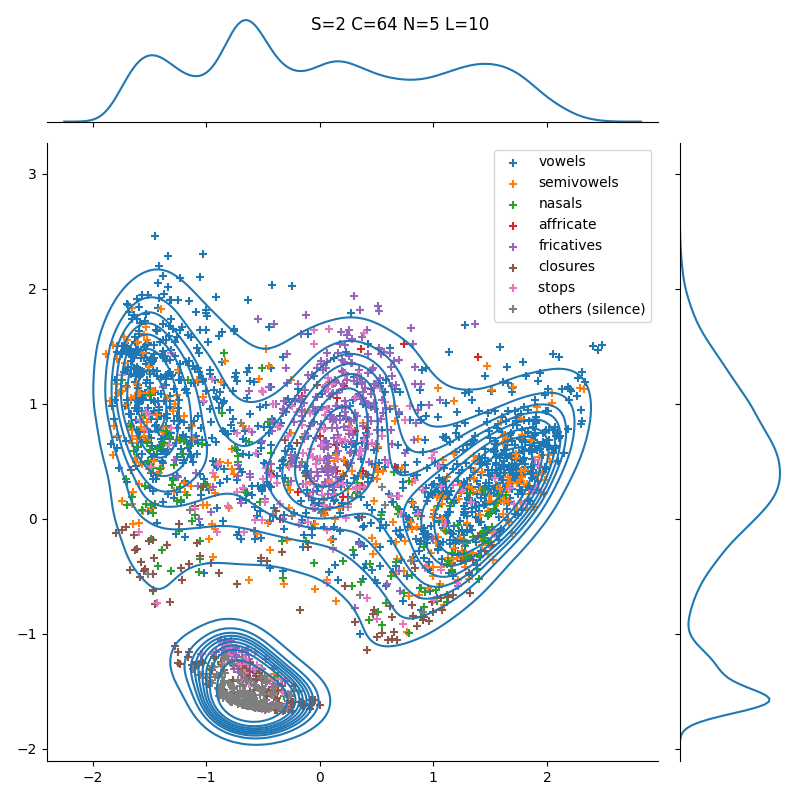
\includegraphics[width=0.5\columnwidth]{ 
        latent_exploration_PCA_S=2_C=64_N=5_L=10.png}%
    % }
    % \subfloat{
        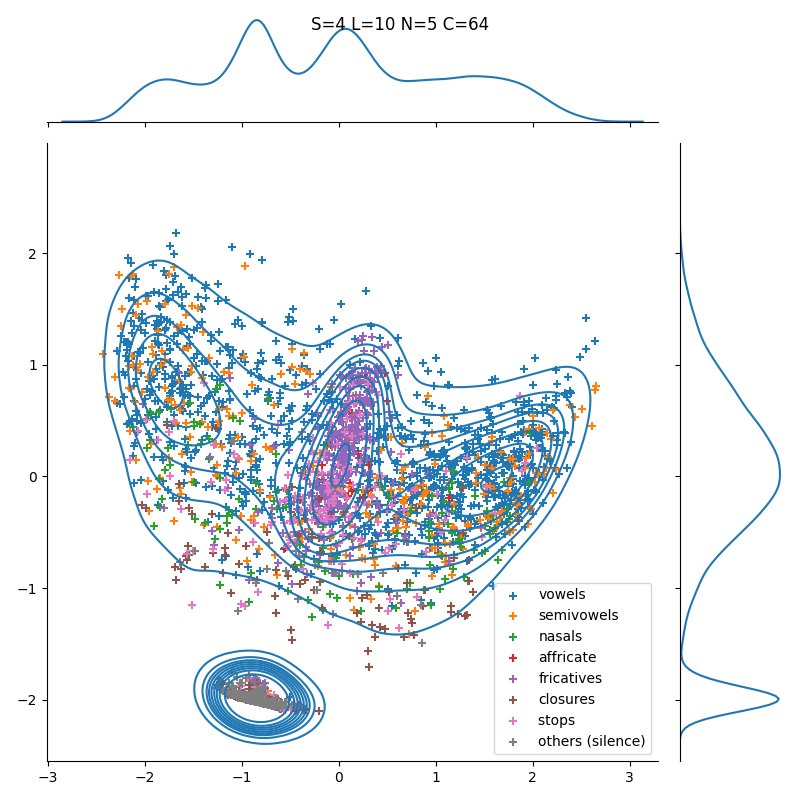
\includegraphics[width=0.5\columnwidth]{ 
        latent_exploration_PCA_S=4_L=10_N=5_C=64.png}%
    % }
    % \subfloat{
    \\
        \includegraphics[width=0.5\columnwidth]{
        % latent_exploration_PCA_S=8_C=64_N=5_L=10.png
        latent_exploration_PCA_S=8_C=64_N=5_L=10.png
        }%
    % }
    % \subfloat{
        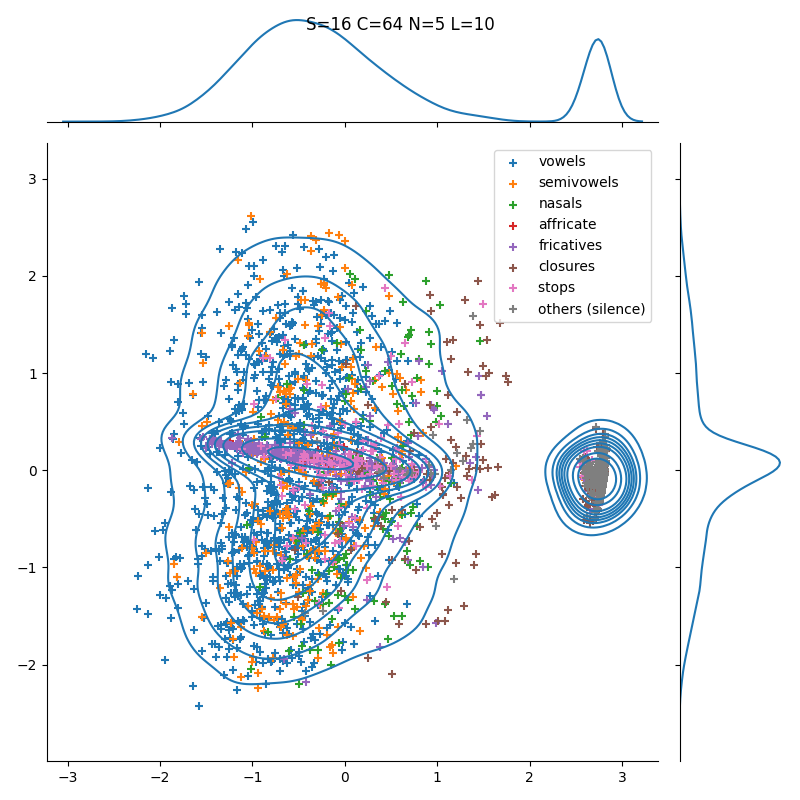
\includegraphics[width=0.5\columnwidth]{
        latent_exploration_PCA_S=16_C=64_N=5_L=10.png
        }%
    % }
    
    \caption{PCA reduction of the latent space of stacked WaveNets with different stack sizes: Top left: 2, Top right: 4, Bottom left: 8, Bottom right: 16}
    \label{fig:wavenet-lat}
\end{figure}


To assess hypothesis \ref{asmpt:represent}, we examined the representations learned by WaveNets with stack sizes $S={2, 4, 8, 16}$ and $R=64$, as reported in \cref{tab:stack-bpds}.
The representations were selected as the output from the residual stack. We pooled all samples from the test set before reducing the dimensionality to 2 dimensions with Principal Components Analysis (PCA). 
We plotted the density of all data points transformed with PCA in \cref{fig:wavenet-lat}. We use phoneme annotations supplied with the TIMIT dataset to overlay 2500 individual representations colored according to the phonemes. The phoneme annotation is selected as the one with highest overlap with the corresponding input segment.
If the WaveNet captures any semantic info, we expect to see phonemes cluster within the linear subspace obtained from PCA. 


For stack size 2 (\cref{fig:wavenet-lat}, top left), we see four explicit nodes, with distinct groups of phonemes in each node.
We observe a clearly separable node, predominantly populated by the \texttt{epi} and \texttt{pau} silence phonemes.
In addition, we observe three large nodes, with vowels and nasals distributed to the two extremes, and the middle node containing most of the affricate, fricative, and stop phonemes.
The same trend is observed in the larger stacks (4,8,16), although with a more smooth density as the stack size increases.
We attribute the increased smoothness of the latent representations as stack size increases higher probability of phoneme overlap within the range of $S$ frames, as $S$ grows.
Nevertheless, this property of the WaveNet supports hypothesis \ref{asmpt:represent}; that WaveNet extracts semantically relevant features in audio.
This builds a case for using WaveNet in semi-supervised learning, like Automatic Speech Recognition (ASR) tasks. 
We explore this hypothesis in \cref{ssec:results-asr}.


\subsection{WaveNet as a Language Model}\label{ssec:results-lm}
To address hypothesis \ref{asmpt:lang-mod}, we designed an experiment for character-level language modeling with the WaveNet. 
To be used for end2end speech generation, WaveNets need to learn to model both low-level features abd high-level features of speech. 
Language modeling experiments allow us to assess the suitability of a WaveNet for these higher-level modeling tasks, using text as a representation of speech.
% TODO: add figure? 
Previously, convolutional language models have surpassed first standard RNNs (\cite{pham_convolutional_2016}) and later RNNs with LSTMs for language modeling
\cite{dauphin_language_2017}.
Notably, Bai and collaborators found Temporal Convolutional Networks, a modified form WaveNets, to outperform LSTMs, GRUs, and RNNs for character-level language modeling
\cite{bai_empirical_2018}.

We implemented the WaveNet as a character-level language model and replaced the DMoL with a categorical distribution over the output tokens. 
We used a shallower architecture with a receptive field of 126 characters to better match the length of a typical sentence. 
\Cref{tab:wavenet_lm} shows the results, where we observe an improvement up to 32 residual channels. 
Compared to other state-of-the-art models, the WaveNet remains below the bar, most notably far below the Temporal Convolutional Network, which contains a similar residual stack of dilated convolutions.
This contradicts hypothesis \ref{asmpt:lang-mod}, and hints that the limiting factor in using a WaveNet for speech synthesis originates from its limits in modeling sequences of latent representations in audio.  

\begin{table}[htb]
    \centering
    \begin{tabular}{l|c||c}
        Model & Dataset & BPD (test) \\
        \hline
        Mogrifier LSTM \cite{melis_mogrifier_2020} & PTB & 1.083 \\
        Temporal Convolutional Network \cite{bai_empirical_2018} & PTB & 1.31 \\
        \hline
        WaveNet N=5 L=4 R=24 [RF 126] & PTB & 1.835 \\
        WaveNet N=5 L=4 R=32 [RF 126] & PTB & \textbf{1.666} \\
        WaveNet N=5 L=4 R=48 [RF 126] & PTB & 1.678 \\
        % WaveNet L=4 N=5 R=64 [RF 126] & Billion Word & 1.483 \\%1.677 \\
    \end{tabular}
    \caption{
    Results of using WaveNet as a character-level language model. 
    State-of-the-art results are shown above for comparison. 
    }
    \label{tab:wavenet_lm}
\end{table}


\subsection{Examining the semantic content of WaveNet representations trained on raw waveforms}\label{ssec:results-asr}
The bits-per-dim metric in \cref{eq:bpd} contains equal contributions from each audio waveform sample. 
As mentioned in \cref{ssec:data-modality}, WaveNets are unable to model intra-step correlation when simultaneously predicting $S$ steps in the future. 
This makes errors in modeling local dependencies more likely, which result in a noisy output signal. 
As the BPD metric measures the likelihood of the data, it will be susceptible to give high BPD values to a noisy signal.
The model's ability to model longer-term semantic information can therefore be masked by high levels of noise.


To establish whether WaveNets capture useful semantic information from raw audio (hypothesis \ref{asmpt:represent}), we designed an experiment for Automatic Speech Recognition (ASR) on the outputs of trained WaveNet models.
First, we trained a WaveNet model with stacking on the \texttt{clean\_100} subset of the Librispeech dataset \cite{noauthor_librispeech_nodate}.
The model uses stacking as described in \cref{data:eq-transform}, with $S=8$, 32 residual channels, and 5 blocks of 10 layers with dilation cycles as described in \cref{tab:stack-bpds}. This makes a receptive field of 40936 frames or 2560 ms of 16 kHz audio. % https://wandb.ai/vseq/wavenet/runs/5nbuqtku/
The model trained until convergence and reached a BPD value of 12.368. %(150 epochs?)

% TODO: introduce CTC loss?
% \cref{tab:wavenet_libri_100h}. 
We then trained an LSTM-based ASR model with Connectionist Temporal Classification (CTC) loss on the outputs of the residual stack of the WaveNet, as shown in \cref{fig:wavenet-asr}
\cite{graves_connectionist_nodate, hochreiter_long_1997}.
The model uses a convolution layer to downsample the input to the LSTM cell to 50 Hz. 
For an 8-stacked model this corresponds to a downsampling factor of 20.

We train a total of seven different model configurations. 
The first five models train on the outputs of the first 10, 20, 30, 40, and 50 layers in WaveNet's residual stack, respectively. 
We also train two baselines. One baseline model trains directly on the stacked raw audio waveform (passed through a convolutional downsampling), as shown in \cref{fig:lstm-asr}.
The second is a single layered LSTM trained on 80-dimensional log-mel spectrograms with window length and hop length set to 320 (20 ms), so as to correspond to 50 Hz. This representation is commonly used for speech modeling and ASR.
% TODO: cite spectrogram
We train the ASR models on different amounts of subsets of the Librispeech \texttt{clean} subset - 10 minutes, 1 hour, and 10 hours, to assess the effect of using WaveNet as a preprocessor in resource settings.

This approach allows us to compare whether the information captured by the lower layers of the WaveNet are \textit{more} valuable than the information that flows through the entire network. 
We evaluated all of these models against the entire \texttt{clean-test} subset for comparability.
From these results, summarized in \cref{tab:wavenet_asr_libri}, we see the following:
\begin{enumerate}
    \item Using WaveNet as a preprocessor decreases the loss when trained on the 1 hour and 10-hour training subsets. 
    \item The best performance occurs when using 30 layers of the WaveNet trained on 10 hours of training data.
    \item Notably, WaveNet's use as a preprocessor grows more competitive when increasing the training data size. 
\end{enumerate}


\begin{figure}
    \centering
    \begin{subfigure}[b]{0.5\linewidth}
        \resizebox{\columnwidth}{!}{
            \begin{tikzpicture}
%% WaveNet Structure first


%% 


\node[circle,draw,fill=blue!50,minimum height=5mm,] (Input-15) at (15,0) {};
\node[circle,draw,fill=gray!30,minimum height=5mm, ] (Hidden1-15) at (15,2) {};
\node[circle,draw,fill=gray!30,minimum height=5mm] (Hidden2-15) at (15,4) {};
\node[circle,draw,fill=gray!30,minimum height=5mm] (Hidden3-15) at (15,6) {};
\node[circle,draw,fill=yellow!50,minimum height=5mm] (Output-15) at (15,8) {};



\draw[->, line width=1.5] (15,0.3) -- (15, 1.7);
\draw[->, line width=1.5] (15,2.3) -- (15, 3.7);
\draw[->, line width=1.5] (15,4.3) -- (15, 5.7);
\draw[->, line width=1.5] (15,6.3) -- (15, 7.7);



\foreach \x in {14, 13, ...,0}{
    \node[circle,draw,fill=blue!50,minimum height=5mm] (Input-\x) at (\x,0) {};
    \node[circle,draw,fill=gray!30,minimum height=5mm] (Hidden1-\x) at (\x,2) {};
    \node[circle,draw,fill=gray!30,minimum height=5mm] (Hidden2-\x) at (\x,4) {};
    \node[circle,draw,fill=gray!30,minimum height=5mm] (Hidden3-\x) at (\x,6) {};
    \node[circle,draw,fill=yellow!30,minimum height=5mm] (Output-\x) at (\x,8) {};
}



\foreach \x in {0, 1, ..., 14}{
	\ifthenelse{\intcalcMod{\x}{2}=0}{
		\draw[->, line width=1.5] (Input-\x) -- (Hidden1-\intcalcAdd{\x}{1});
		\draw[->, line width=.5,dashed] (Input-\x) -- (Hidden1-\x);
	}{
		\draw[->, line width=1.5] (Input-\x) -- (Hidden1-\x);
		\draw[->, line width=.5, dashed] (Input-\x) -- (Hidden1-\intcalcAdd{\x}{1});
	}
	\ifthenelse{\intcalcMod{\x}{4}=1}{
   		\draw[->, line width=1.5] (Hidden1-\x) -- (Hidden2-\intcalcAdd{\x}{2});
	}{
	    \ifnodedefined{Hidden2-\intcalcAdd{\x}{2}}{
   		\draw[->, line width=.5, dashed] (Hidden1-\x) -- (Hidden2-\intcalcAdd{\x}{2});
   		}{}
	}
	\ifthenelse{\intcalcMod{\x}{4}=3}{
   		\draw[->, line width=1.5] (Hidden1-\x) -- (Hidden2-\x);
	}{
       	\draw[->, line width=.5,dashed] (Hidden1-\x) -- (Hidden2-\x);
	}
	\ifthenelse{\intcalcMod{\x}{8}=3}{
		\draw[->, line width=1.5] (Hidden2-\x) -- (Hidden3-\intcalcAdd{\x}{4});
	}{
        \ifnodedefined{Hidden3-\intcalcAdd{\x}{4}}{
   		    \draw[->, line width=.5, dashed] (Hidden2-\x) -- (Hidden3-\intcalcAdd{\x}{4});
   		}{}
	}
	\ifthenelse{\intcalcMod{\x}{8}=7}{
   		\draw[->, line width=1.5] (Hidden2-\x) -- (Hidden3-\x);
	}{
   		\draw[->, line width=.5, dashed] (Hidden2-\x) -- (Hidden3-\x);
	}
	\ifthenelse{\intcalcMod{\x}{16}=7}{
		\draw[->, line width=1.5] (Hidden3-\x) -- (Output-\intcalcAdd{\x}{8});
	}{
	\ifnodedefined{Output-\intcalcAdd{\x}{8}}{
   		    \draw[->, line width=.5, dashed] (Hidden3-\x) -- (Output-\intcalcAdd{\x}{8});
   		}{}
	}
	\ifthenelse{\intcalcMod{\x}{16}=15}{
   		\draw[->, line width=1.5] (Hidden3-\x) -- (Output-\x);
	}{
	\draw[->,  line width=.5, dashed] (Hidden3-\x) -- (Output-\x);
	}
}



%% Convolutional Layer

\node[rectangle, draw, rounded corners, above=of Output-15] (Conv-15)  {Conv1D};
\node[rectangle, draw, rounded corners, above=of Output-11] (Conv-11)  {Conv1D};
\node[rectangle, draw, rounded corners, above=of Output-7] (Conv-7)  {Conv1D};
\node[rectangle, draw, rounded corners, above=of Output-3] (Conv-3)  {Conv1D};

\foreach \x in {0, 1, ..., 15}{
\ifthenelse{
    \intcalcMax{\x}{3}=3
}{
    \draw[->, line width=1.5] (Output-\x) -- (Conv-3);
}{
\ifthenelse{
    \intcalcMax{\x}{7}=7
}{
    \draw[->, line width=1.5] (Output-\x) -- (Conv-7);
}{
\ifthenelse{
    \intcalcMax{\x}{11}=11
}{
    \draw[->, line width=1.5] (Output-\x) -- (Conv-11);
}{

    \draw[->, line width=1.5] (Output-\x) -- (Conv-15);
}
}
}
}

\foreach \i in {3,7,11,15}{
\node[rectangle, draw, above=of Conv-\i, minimum height=1cm, minimum width=1cm] (LSTM-\i) {LSTM};
\node[circle, minimum size = 10mm, draw, fill=gray!30, above=of LSTM-\i] (X-hat-\i) {$\hat{x}$};
\draw[->, line width=1.5] (Conv-\i) -- (LSTM-\i);
\draw[->, line width=1.5] (LSTM-\i) -- (X-hat-\i);
\ifthenelse{\i=3}{!}{
\draw[->] (LSTM-\intcalcSub{\i}{4}) -- (LSTM-\i) node[midway, above] {$h_t$};
}
}


\node[above=of X-hat-3] (Text-3) {R};
\node[above=of X-hat-7] (Text-7) {A};
\node[above=of X-hat-11] (Text-11) {I};
\node[above=of X-hat-15] (Text-15) {N};

\draw[->] (X-hat-3) -- (Text-3) {};
\draw[->] (X-hat-7) -- (Text-7) {};
\draw[->] (X-hat-11) -- (Text-11) {};
\draw[->] (X-hat-15) -- (Text-15) {};

% Text and notes
\node[right=of Input-15, align=left] {
\textbf{Input}
};
% \node[right=of Hidden1-15, align=left] {
% \textbf{Hidden1}\\
% Dilation = 1
% };
\node[right=of Hidden2-15, align=left] {
\textbf{Hidden Layers}\\
};
% \node[right=of Hidden3-15, align=left] {
% \textbf{Hidden3}\\
% Dilation = 4
% };
\node[right=of Output-15, align=left] {
\textbf{WaveNet Output}\\
};

\node[right=of Conv-15, align=left] {
\textbf{Convolutional}\\\textbf{Downsampler}
};

\node[right=of LSTM-15, align=left] {
\textbf{LSTM}\\\textbf{ASR Model}
};

\node[right=of X-hat-15, align=left] {
\textbf{Softmax Output}
};

\node[right=of Text-15, align=left] {
\textbf{Decoded Output}
};

\end{tikzpicture}
        }
    \caption{Setup of the WaveNet-LSTM ASR experiment.}
    \label{fig:wavenet-asr}
    \end{subfigure}%
    \begin{subfigure}[b]{0.5\linewidth}
        \resizebox{\columnwidth}{!}{
            \begin{tikzpicture}
    % Input
    \foreach \x in {0, 1, ..., 15}{
            \node[circle,draw,fill=blue!50,minimum height=5mm] (Input-\x) at (\x,0) {};
        }

    %% Convolutional Layer

    \node[rectangle, draw, rounded corners, above=of Input-15] (Conv-15)  {Conv1D};
    \node[rectangle, draw, rounded corners, above=of Input-11] (Conv-11)  {Conv1D};
    \node[rectangle, draw, rounded corners, above=of Input-7] (Conv-7)  {Conv1D};
    \node[rectangle, draw, rounded corners, above=of Input-3] (Conv-3)  {Conv1D};

    \foreach \x in {0, 1, ..., 15}{
            \ifthenelse{
                \intcalcMax{\x}{3}=3
            }{
                \draw[->, line width=1.5] (Input-\x) -- (Conv-3);
            }{
                \ifthenelse{
                    \intcalcMax{\x}{7}=7
                }{
                    \draw[->, line width=1.5] (Input-\x) -- (Conv-7);
                }{
                    \ifthenelse{
                        \intcalcMax{\x}{11}=11
                    }{
                        \draw[->, line width=1.5] (Input-\x) -- (Conv-11);
                    }{

                        \draw[->, line width=1.5] (Input-\x) -- (Conv-15);
                    }
                }
            }
        }

    \foreach \i in {3,7,11,15}{
            \node[rectangle, draw, above=of Conv-\i, minimum height=1cm, minimum width=1cm] (LSTM-\i) {LSTM};
            \node[circle, minimum size = 10mm, draw, fill=gray!30, above=of LSTM-\i] (X-hat-\i) {$\hat{x}$};
            \draw[->, line width=1.5] (Conv-\i) -- (LSTM-\i);
            \draw[->, line width=1.5] (LSTM-\i) -- (X-hat-\i);
            \ifthenelse{\i=3}{!}{
                \draw[->] (LSTM-\intcalcSub{\i}{4}) -- (LSTM-\i) node[midway, above] {$h_t$};
            }
        }

    \node[above=of X-hat-3] (Text-3) {R};
    \node[above=of X-hat-7] (Text-7) {A};
    \node[above=of X-hat-11] (Text-11) {I};
    \node[above=of X-hat-15] (Text-15) {N};

    \draw[->] (X-hat-3) -- (Text-3) {};
    \draw[->] (X-hat-7) -- (Text-7) {};
    \draw[->] (X-hat-11) -- (Text-11) {};
    \draw[->] (X-hat-15) -- (Text-15) {};

    % Text and notes
    \node[right=of Input-15, align=left] {
        \textbf{Input}
    };

    \node[right=of Conv-15, align=left] {
        \textbf{Convolutional}\\\textbf{Downsampler}
    };

    \node[right=of LSTM-15, align=left] {
        \textbf{LSTM}\\\textbf{ASR Model}
    };

    \node[right=of X-hat-15, align=left] {
        \textbf{Softmax Output}
    };

    \node[right=of Text-15, align=left] {
        \textbf{Decoded Output}
    };

\end{tikzpicture}
        }
    \caption{Setup of the LSTM ASR experiment.}
    \label{fig:lstm-asr}
    \end{subfigure}
    \caption{
    Comparison of the WaveNet-LSTM and LSTM ASR experiment setups.
    }
\end{figure}



\begin{table}[tb]
    \centering
    \begin{tabular}{c||c|c|c}
         Model & CER (Loss) - 10min & CER (Loss) - 1h & CER (Loss) - 10h \\
         \hline\hline
         LSTM & 1.00 (1625.7) & 0.691  (1463.7) & 0.6050 (1131.9)  \\ % https://wandb.ai/vseq/wavenet_asr/runs/2czd2qia
         LSTM + Spectrogram & 0.75 (1331.7) & 0.56 (1042.2) & 0.465 (825.7) \\ %
         % https://wandb.ai/vseq/wavenet_asr/runs/qg6nbvq7/
         % https://wandb.ai/vseq/wavenet_asr/runs/1776h0c9/
         % https://wandb.ai/vseq/wavenet_asr/runs/11uixeag/
         \hline
         LSTM+WaveNet-10 & 1.0    (1611.8) & 0.7066 (1457.1) & 0.5122 (927.9) \\
         LSTM+WaveNet-20 & 0.9965 (1615.0) & 0.7969 (1527.3) & 0.4618 (862.3) \\
         LSTM+WaveNet-30 & 0.9983 (1634.1) & 0.8681 (1502.5) & \textbf{0.4184 (800.5)} \\
         LSTM+WaveNet-40 & 0.9983 (1632.0) & 0.7326 (1463.5) & 0.4392
 (815.5) \\
         LSTM+WaveNet-50 & 0.9983 (1645.8) & \textbf{0.6701 (1326.2)} & 0.4757 (870.0)\\
    \end{tabular}
        \caption{Comparisons of ASR models with and without pretrained WaveNet transformations on the input signal.
        Models are trained, respectively, with 10 minutes, 1 hour, and 10 hours of training data. 
        CTC Loss and CER are reported on the Librispeech \texttt{clean-test} subset.
        }
        \label{tab:wavenet_asr_libri}
\end{table}


\iffalse
\subsection{Testing WaveNet's capabilities at protein sequence modelling.}\label{ssec:proteins}
Following the methodology of the Debbie Marks' lab, we probed whether our implementation of WaveNet is suitable for modelling protein sequences. \cite{shin_protein_2021}
We trained WaveNets similar to the ones presented in \cref{ssec:results-lm}

\textit{[Results still pending]}
\fi

% \begin{table}[tb]
% \centering
%     \begin{tabular}{c|c}
%         Stack size & BPD \\
%         \hline
%       8 & 12.368 \\ 
%       4 & 12.466 \\
%       % TODO: get 1 stack for comparison with Jakob
%     \end{tabular}
    
%     \caption{
%         BPDs for WaveNet models trained on the \texttt{clean\_100} subset of the Librispeech, and evaluated on the Librispeech \texttt{clean} test set.    
%         Models have 32 residual channels and 5 blocks of 10 layers with dilation cycles as described in \cref{tab:stack-bpds}. 
%     }
%     \label{tab:wavenet_libri_100h}
% \end{table}
